\chapter{Erkennung der Cry-Units}
\label{sec:vad}

Der erste notwendige Schritt zur Ableitung einer Pain Score aus einem Audiosignal ist die Feststellung, ob in dem Signal überhaupt kindliche Lautäußerungen vorhanden sind. Das Ziel ist, in einem Audiosignal diejenigen Bereiche zu markieren, in denen Stimmaktivität vorhanden ist und daraufhin Beginn und Ende der einzelnen Cry-Units zu festzulegen. Abbildung  \ref{img:vad01} verdeutlicht diese Aufgabe an einem Beispiel: Der obere Graph zeigt in Schwarz ein Audiosignal. Die rote Linie, die das Signal überspannt, zeigt, welche Regionen Stimme enthalten, wobei $1 \hat{=} $ \emph{stimmhaft} (engl. \emph{voiced}) und $0 \hat{=}  $ \emph{nicht stimmhaft} (oder \emph{Stille}, engl. \emph{not voiced}). Das untere Schema zeigt, wie die stimmhaften Signalbereiche zu Cry-Units zusammengefasst wurden.

\begin{figure}[h]
	\centering
	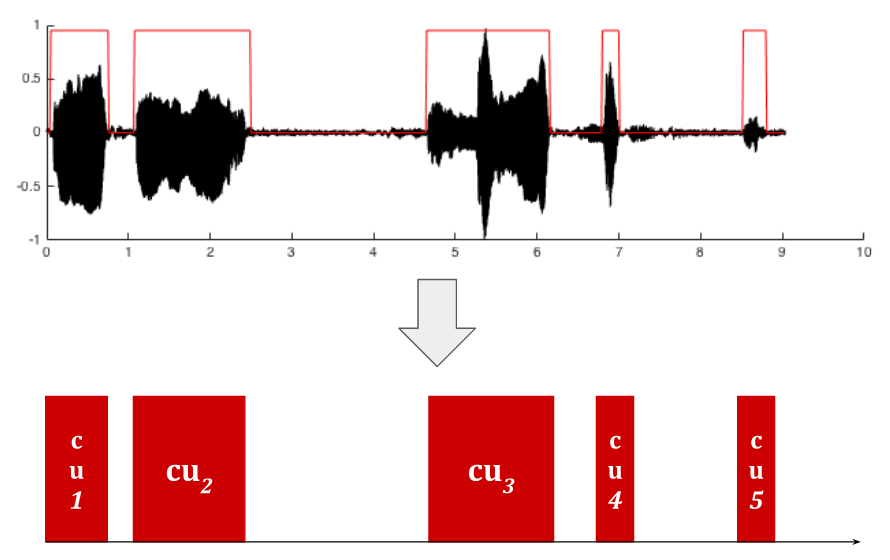
\includegraphics[width=0.7\textwidth]{bilder/vad_introduction02.png}
	\caption{Markierung stimmhafter Bereiche in einem Audiosignal. Oben Schwarz: Das Eingangssignal $x[\;]$. Oben Rot: Klassifizierung in stimmhaft/Stille. Unten Rot: Die fünf erkannten Cry-Units.}
	\label{img:vad01}
\end{figure}

In Kapitel \ref{sec:vad_new} wird die Voice Activity Detection vorgestellt, das Feststellen des Vorhandenseins von Stimme in einem Signal. In Kapitel \ref{sec:marking_cry-units_new} wird besprochen, wie die stimmhaften Signalbereiche zu Cry-Units zusammengefasst werden. In Kapitel \ref{sec:decision_smoothing_new} wird ein Algorithmus vorgestellt, in dem Nachträglich inkorrekt erkannte Anfangs- und Endzeitpunkt von Cry-Units korrigiert werden.

\section{Voice Activity Detection}
\label{sec:vad_new}

\emph{Voice Activity Detection} (kurz \emph{VAD}) oder \emph{Speech Detection} ist bei jeder Art der Sprachverarbeitung von Bedeutung: Im Mobilfunk wird sie beispielsweise eingesetzt, um die Zeitbereiche zu Erkennen, in denen die Teilnehmer sprechen und somit eine Übertragung stattfinden muss. Die größte Herausforderung von VAD-Systemen ist die robuste Erkennung von Stimmaktivität auch bei starkem Hintergrundrauschen. Bis heute wurde keine \glqq perfekte Lösung\grqq{} des Problems gefunden. \cite[S. 1]{vad_granada} \cite[S. 1]{vad_kola} \cite[S. 1]{vad_Lisboa}

Der Grundlegende Aufbau eines VAD-Algorithmus ist wie folgt. Abbildung \ref{img:vad_pipeline} visualisiert diesen Aufbau.
\begin{enumerate}
	\item \textbf{Vorverarbeitung} (engl. Pre-Proccessing) des Signals.
	\item \textbf{Windowing: } Unterteilung des Signals in (einander überlappende) Signalfenster.
	\item \textbf{Extraktion von Eigenschaften} (engl. \emph{Feature-Extraction}) aus jedem Signalfenster.
	\item \textbf{Entscheidung} (engl. \emph{Decision}) über die Präsens oder Abwesenheit von Stimme für jedes Signalfenster auf Grundlage der extrahierten Eigenschaften
	\item \textbf{Decision-Smoothing}, das nachträgliche Hinzufügen oder Entfernen von Entscheidungen mit Hilfe kontextueller Informationen der umliegenden Entscheidungen.\cite[S. 8 - 9]{vad_granada} \cite[S. 1 - 2]{vad_kola}
\end{enumerate}

\begin{figure}[h]
	\centering
	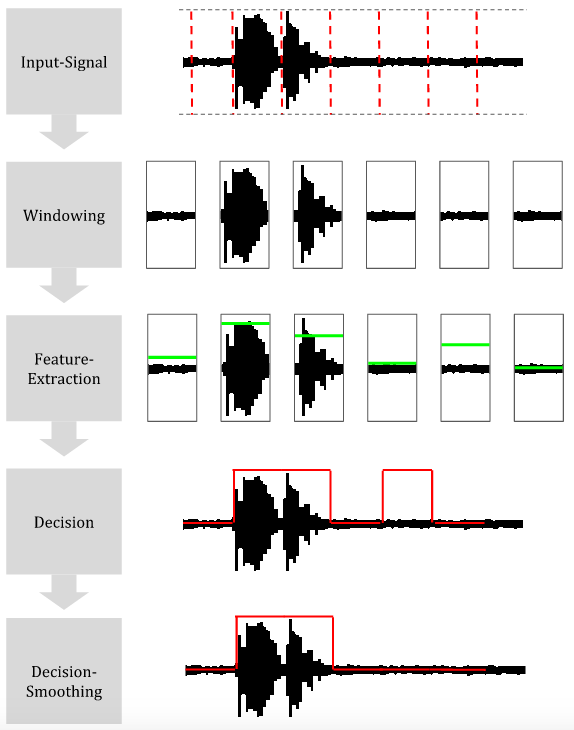
\includegraphics[width=0.65\textwidth]{bilder/vad_pipeline03.png}
	\caption{Aufbau eines VAD-Algorithmus}
	\label{img:vad_pipeline}
\end{figure}


In Kapitel \ref{sec:methods_vad_new} werden die Methoden vorgestellt, die zur Voice Activity Detection erprobt wurden. In Kapitel \ref{sec:vad_study} wird eine Simulationsstudie beschrieben, deren Ziel die Bestimmung derjenigen Methoden war, die sich für die VAD im speziellen Fall kindlicher Lautäußerungen am besten eignen. Kapitel \ref{sec:vad_results} fasst die Ergebnisse zusammen.

\subsection{Methoden}
\label{sec:methods_vad_new}

Die in diesem Kapitel vorgestellten Methoden kombinieren Ideen, die von Moattar et al. \cite{vad_Easy}, Kristjansson et al. \cite{vad_Lisboa}, Waheed et al. \cite{vad_entropy}, Ahmadi et al. \cite{vad_ceps} und Shen et al.\cite{vad_entropie02} vorgestellt wurden.

\subsubsection{Vorverarbeitung}
\label{sec:preprocessing}

Bei der Vorverarbeitung wird das Signal so manipuliert, dass Störeinflüsse auf die darauf folgenden Verarbeitungsschritte minimiert werden. Welche Vorverarbeitung durchgeführt wird, ist Abhängig von der konkreten Aufgabenstellung. Dieser Schritt ist für die VAD optional. So setzten beispielsweise Ahmadi et al. \cite{vad_ceps} einen Bandpassfilter bei der Vorverarbeitung ein, während Moattar et al. \cite{vad_Easy} keine Vorverarbeitung anwendeten. 

In dieser Arbeit sich für eine Vorverarbeitung entschieden, bei der das Signal hinsichtlich seiner Dynamik im Zeitbereich eingeschränkt wird. Dies ist ein typischer Vorverarbeitungsschritt bei Sprachaufnahmen. So wird vermieden, dass ein Signal eventuell zu leise ist, damit überhaupt Etwas darin erkannt werden kann. Einer der hauptsächlichen Gründe, warum ein Signal eine niedrige durchschnittliche Energie aufweisen kann, obwohl es maximal ausgesteuert wurde, sind sehr kurze Pegelspitzen, deren Pegel weit über dem Durchschnittspegel liegen und so eine weitere Erhöhung der Lautstärke verhindern. Da die Audiosignale, die in der in Kapitel \ref{sec:vad_study} vorgestellten Simulationsstudie verwendet wurden, aus inhomogenen Quellen stammen und sehr unterschiedliche Lautstärken hatten, wurde so eine Angleichung der Signalenergien gewährleistet.

Die Dynamikeinschränkung wurde mit Hilfe eines Audio-Kompressors umgesetzt. Dieser verringert Signalspitzen, die über einen festgelegten \emph{Schwellwert} (engl. \emph{Threshold}) $\theta$ liegen, um ein festgelegtes \emph{Verhältnis} (engl. \emph{Ratio)} $\rho$. Ein Schwellwert von $\theta = 0.3$ mit einem Verhältnis von $\rho = 0.5$ bedeutet beispielsweise, dass alle Signalspitzen, die den Wert 0.3 über-, oder $-0.3$ unterschreiten, um 50\% verringert werden. Der Wert eines Samples nach der Kompression $x_{comp}[n]$ ergibt sich somit nach Gleichung \ref{eq:preprocessedX}.

\begin{equation}
\text{comp}(x[n], \theta, \rho) =
\begin{cases}
\theta + (x[n] - \theta) \rho \quad , \text{wenn } x[n] > \theta \\
-\theta + (x[n] + \theta) \rho \quad, \text{wenn } x[n] < -\theta \\
x[n] \quad \text{sonst}
\end{cases}
\label{eq:preprocessedX}
\end{equation}

Die Amplituden hoher Signalspitzen werden so verringert, wodurch Headroom gewonnen wird, welcher anschließend bei der gleichmäßigen Erhöhung aller Amplituden zur Erhöhung der insgesamten Energie genutzt werden kann. Diese Erhöhung kann beispielsweise durch eine Normalisierung nach Gleichung \ref{eq:normalizing} durchgeführt werden.

\begin{equation}
\text{normalize}(x[n]) = \frac{x[n]}{\maxi\{x[\;]\}}
\label{eq:normalizing}
\end{equation}

Bei dem Kompressor, der in dieser Verarbeitungs-Pipeline zur Vorverarbeitung verwendet wird, werden Threshold und Ratio nach Formel \ref{eq:THold} als Funktion des RMS-Wertes des Signals berechnet. Der Parameter $r_a$ gibt den Ziel-RMS-Wert an. Der RMS-Wert wird nach Formel \ref{eq:rms} berechnet.

\begin{equation}
\theta(x[\;]) = \rho(x[\;])  = \bigg[\frac{\text{RMS}(x[\;])}{r_a}\bigg]^{2}
\label{eq:THold}
\end{equation}

Die Vorverarbeitung wurde durchgeführt, indem 1.) die Kompression mit den Parametern nach Gleichung \ref{eq:THold} und 2.) die Normalisierung nach Gleichung \ref{eq:THold} durchgeführt wurde. Abbildung \ref{img:compressing01} zeigt ein Signal vor und nach der Vorverarbeitung nach diesem Prinzip. Um eine zu große Beeinflussung des Signals zu vermeiden, wurde ein Minimalwert für Threshold und Ratio von $0.4$ festgelegt.

\begin{figure}[h]
	\centering
	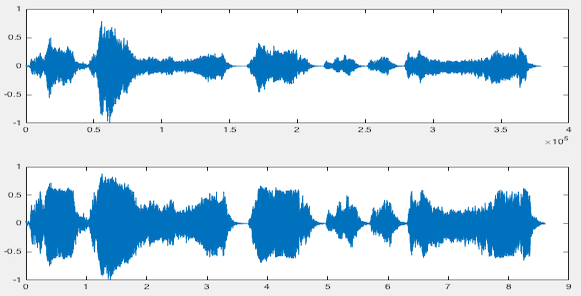
\includegraphics[width=0.7\textwidth]{bilder/compressing01.png}
	\caption{Ergebnis der Vorverarbeitung. Oben: Das Signal vor der Vorverarbeitung. Unten: Das Signal nach der Vorverarbeitung.}
	\label{img:compressing01}
\end{figure}

Diese Vorverarbeitung eignet sich nicht für ein kontinuierliches System, da Samples zur Berechnung des RMS-Wertes mit einbezogen werden, die zu einem Berechnungszeitpunkt in der Zukunft liegen. Das Hauptziel dieser Vorverarbeitung war die Herstellung ähnlicher Energieverhältnisse bei den Signalen, die in der Simulationsstudien in Kapitel \ref{sec:vad_study} verwendet wurden. Damit diese Vorverarbeitung in einem kontinuierlichen System eingesetzt werden kann, wird die folgende Abwandlung vorgeschlagen:
\begin{itemize}
	\item Komplettes Überspringen der Vorverarbeitung, in dem mit Hilfe eines manuell einstellbaren Lautstärkereglers eine ausreichende Signalenergie gewährleistet wird. Würde man beispielsweise anstelle der Analyse des Audiosignals das Gesicht des Neugeborenen mit einer Kamera untersuchen, würde man ebenfalls eine ausreichende Bildhelligkeit voraussetzen.
	\item Die Initialisierung des Kompressor mit \grqq sanften Werten\grqq , wie zum Beispiel $\theta = \rho = 0.7$ und $\maxi\{x[\;] = 0.9\}$. Diese Parameter können nach der Beendigung eines Segmentes (Siehe Kapitel \ref{sec:segmenting}) auf Basis des RMS-Wertes des Segmentes aktualisiert und für die Vorverarbeitung der zukünftigen Werte eingesetzt werden.
\end{itemize}

\subsection{Windowing}
\label{sec:windowing}

Angenommen, man führt die Voice Activity Detection für das Signal $x[\;]$ durch und kommt zu dem Schluss, dass in dem Signal (teilweise) Stimme enthalten ist. Ist das Signal mehrere Minuten oder sogar Stunden lang, ist allein aus der Entscheidung nicht ersichtlich, in welchen Zeitbereichen genau Stimme enthalten ist, und in welchen nicht. Um die zeitliche \glqq Auflösung\grqq{} zu erhöhen, wird das Signal in kürzere Zeitfenster zerlegt.

Nach der Vorverarbeitung wird diese Zerlegung mit Hilfe der in Kapitel \ref{sec:stft} als \emph{Windowing} bezeichneten Methode durchgeführt. Das Signal $x[\;]$ wird nach Gleichung \ref{eq:signal-Window} in die Signalfenster $x_0[\;] , \ldots , x_m[\;]$ aufgeteilt. Die Zeitfenster werden zunächst im Zeitbereich belassen. Es wurde sich für die von Waheed et al. \cite{vad_entropy} vorgeschlagene Fensterlänge von \SI{25}{\milli\second} entschieden, als Kompromiss zwischen den von Moattar et al. \cite{vad_Easy} empfohlenen \SI{10}{\milli\second} und den von Ahmadi et al. \cite{vad_ceps} empfohlenen \SI{40}{\milli\second}. Die Fenster überlappen einander um 50\%, das heißt \SI{12.5}{\milli\second}.

Die Entscheidung über das Vorhandensein von Stimme wird \emph{einzeln} für jedes der Signalfenster $x_0[\;] , \ldots , x_m[\;]$ durchgeführt. Grundlage für die Entscheidung ist eine Menge an Features, die für das jeweilige Signalfenster $x_i[\;]$ berechnet wird. Die Erforschung geeigneter Features ist eines der primären Forschungsgegenstände der VAD. In den folgenden Kapiteln \ref{sec:vad_time_features} bis \ref{sec:vad_ceps_features} wird eine Reihe an Features vorgestellt, die in dieser Arbeit zur VAD erprobt wurden. Jedes der in diesen Kapiteln besprochenen Features kann für ein Signalfenster $x_i[\;]$ \`{a} \SI{25}{\milli\second} berechnet werden und als Grundlage für eine Entscheidung dienen. Die Evaluation, welche Eigenschaften sich am besten zur Feststellung von Stimme im speziellen Fall von Neugeborenen eignen, folgt in Kapitel \ref{sec:vad_study}

\subsubsection{Eigenschaften des Zeitbereiches}
\label{sec:vad_time_features}

Im Zeitbereich wurden die beiden Eigenschaften\emph{Root Mean Square} [\emph{RMS}] und \emph{Zero Crossing Rate} [\emph{ZCR}] erprobt.

Moattar et al. \cite{vad_Easy} bezeichnen den Energiegehalt eines Signals als das für die VAD am häufigsten angewandte Attribut. Der RMS-Wert als Feature für ein Signalfenster wurde nach Gleichung \ref{eq:rms} berechnet. Hintergrund ist, dass der Energiegehalt eines Stimmsignals typischerweise höher ist als der des Hintergrundrauschens. Bei geringem Signal/Rausch-Abständen ist diese Bedingung jedoch nicht immer gegeben. Als zweites Attribut des Zeitbereiches wurde die \emph{Zero Crossing Rate} berechnet. Die ZCR nach Formel \ref{eq:zcr} gibt an, wie häufig ein Vorzeichenwechsel im Signal vorkommt. Eine höhere ZCR weist auf ein stimmloses Signal hin, da Rauschen typischerweise eine höhere ZCR als stimmhafte Signale aufweist. Problematisch ist dieses Kriterium bei Signalen, bei denen kein Hintergrundrauschen vorliegt, da sich dort eine ZCR von 0 ergibt.\cite{vad_ceps} Um den Wert in Relation zur Fensterlänge setzen zu können, wurde weiterhin die ZCR durch die Anzahl der Samples eines Signalfensters $N$ geteilt.

\begin{equation}
\text{ZCR}(x_i[\;]) = \sum_{0}^{N-1}|\text{sng}(x_i[n])-\text{sng}(x_i[n-1])|
\label{eq:zcr}
\end{equation}

\subsubsection{Eigenschaften der Autokorrelation}

Neben den in Kapitel \ref{sec:featExtraction} genannten \glqq einfachen\grqq{} Attributen des Zeitbereiches wurde die Autokorrelation zur VAD erprobt. Die Autokorrelation eignet sich, um Periodizität in einem Signal nachzuweisen. Wie in Kapitel \ref{sec:theVoice} ausgeführt, weisen stimmhafte Signale eine tendenziell stärkeres periodisches Verhalten als das Hintergrundrauschen auf. 

Bei der Autokorrelation wird ein Signal mit einer verzögerten Variante von sich selber korreliert. Gleichung \ref{eq:ACorr} definiert die Autokorrelation des $N$-Sample langen Signalfensters $x_i[\;]$, verzögert um das Lag $k$.

\begin{equation}
\text{A-Corr}_k(x[\;]) = \sum_{n=k}^{N} x[n-k] \cdot x[n]
\label{eq:ACorr}
\end{equation}

Da der Autokorrelationswert neben der Periodizität von der Signalenergie abhängig ist, ist eine Normalisierung des Wertes wünschenswert. Es gibt verschiedene Varianten dieser Normalisierung. Gleichung \ref{eq:NACorr} definiert die \glqq normalisierte Autokorrelation\grqq{}, bei der der Autokorrelationswert durch die RMS-Werte des verzögerten und unverzögerten Signals normalisiert wird.\cite{vad_Lisboa}

\begin{equation}
\text{NA-Corr}_k(x[\;]) = \frac{\sum_{n=k}^{N} x[n-k] \cdot x[n]}{ \sqrt{\sum_{n=1}^{N-k}  x[n]^2}  \cdot  \sqrt{\sum_{n=k}^{N}  x[n]^2} }
\label{eq:NACorr}
\end{equation}

Das Autokorrelations-Signal $a[\;]$ wird erstellt, indem die normalisierte Autokorrelation für verschiedene $k = k_{min} , \ldots , k_{max}$ angewandt wird, wie Gleichung \ref{eq:a-Signal} definiert. 

\begin{equation}
a[\;] := \quad \mathop{\forall}_{k = k_{min}}^{k_{max}} :\ a[k] = \text{NA-Corr}_k(x[\;]) 
\label{eq:a-Signal}
\end{equation}

Ein hoher Wert des Signals $a[\;]$ an der Position $k$ spricht für eine ausgeprägte Periodizität des Signals mit der Frequenz $f =  f_s / k $. Es ist üblich, den Bereich $[k_{min},k_{max}]$ so einzuschränken, dass die Autokorrelation nur für den Frequenz-Raum durchgeführt wird, in dem man Periodizität erwartet.\cite{vad_Lisboa}

In Bezug auf die VAD wurde die Autokorrelation wird als Methode genutzt, um die beiden Attribute \emph{höchste Autokorrelationsspitze} [\emph{aMax}] und \emph{Anzahl der Autokorrelationsspitzen} [\emph{aCount}] zu berechnen. Beide Eigenschaften wurden von Kristjansson et al. \cite[S. 1 - 2]{vad_Lisboa} zur VAD beschrieben. Die \emph{höchste Autokorrelationsspitze} wird in Formel \ref{eq:corrpeak} definiert und bestimmt die höchste Magnitude im Autokorrelationssignal. Ein stimmhaftes Signal hat aufgrund seiner Periodizität erwartungsgemäß einen höheren [\emph{aMax}]-Wert als Rauschen.

\begin{equation}
\text{aMax}(x_i[\;]) = \max_{k}\text{mag}\{\text{NA-Corr}_k(x_i[\;])\}
\label{eq:corrpeak}
\end{equation}

Die \emph{Anzahl der Autokorrelationsspitzen} wird nach Formel \ref{eq:corrcount} berechnet. Das Feature gibt an, wie viele Signalspitzen im Autokorrelationssignal enthalten sind. Rauschen erzeugt höhere [\emph{aCount}]-Wert als stimmhafte Signale, bedingt durch die vielen zufällig entstehenden Periodizitäten.
\begin{equation}
\text{aCount}(x_i[\;]) = \counti_{k}\text{mag}\{\text{NA-Corr}_k(x_i[\;])\}
\label{eq:corrcount}
\end{equation}

Aus Kapitel \ref{sec:acousticModel} ging hervor, dass die Grundfrequenz der Stimme von Neugeborenen zwischen $250$ und $\SI{2000}{\hertz}$ liegt, weshalb auch nur in Lags dieses Bereichs bei der Berechnung beider Features verwendet wurden.

\subsubsection{Eigenschaften des Frequenzbereiches}

Aus dem Frequenzbereich wurden die drei Eigenschaften \emph{unnormalisierte spektrale Entropie} [$SEnt_{u}$], \emph{normalisierte spektrale Entropie}  [$SEnt_{n}$] und \emph{dominanteste Frequenzkomponenten} [$f_{dom}$] erprobt.

Als Vorbereitungsschritt muss das Signalfenster des Zeitbereiches $x_i[\;]$ in den Frequenzbereich $X_i[\;]$ transformiert werden. Die Berechnungsvorschrift ist $X_i[\;] = \text{DFT}\{(w[\;] \cdot x_i[\;])\}$. Wird diese Transformation für alle Signalfenster $x_0[\;], \ldots, x_m[\;]$ eines Signals durchgeführt, entspricht dies der in Kapitel \ref{sec:stft} vorgestellten Short Time Fourier Transformation. Es wurde eine $2048$ Punkte Lange FFT und eine Hamming-Window als Fensterfunktion $w[\;]$ verwendet.

Kristjansson et al. \cite[S. 2]{vad_Lisboa} haben die \emph{spektrale Entropie} zur Voice Activity Detection beschrieben. Dabei wird das Spektrum des Frequenzfensters $X_i[\;]$ als Wahrscheinlichkeitsverteilung betrachtet. Die Entropie als Maß zur \glqq Unreinheit\grqq{} wurde in Kapitel \ref{sec:id3} erläutert. Die \emph{normalisierte spektrale Entropie} wird nach der Formel \ref{eq:norm_se} berechnet. Das Signal $px_i[\;]$ ergibt sich durch die Normalisierung des $N$-Punkte langen Spektrums nach Formel. Bei der normalisierten spektralen Entropie ist zu erwarten, dass Frequenzfenster ohne Stimme einen höheren Wert aufweisen als Fenster mit Stimme.\ref{eq:norm_spek}. 

\begin{equation}
px_i[n] = \frac{X_i[n]}{\sum_{k=1}^{N} X_i[k]}
\label{eq:norm_spek}
\end{equation}

\begin{equation}
\text{SEnt}_n(px_i[\;]) = -\sum_{k=1}^{N}px_i[k] \cdot\log(px_i[k])
\label{eq:norm_se}
\end{equation}

Neben der von Kristjansson et al. \cite{vad_Lisboa} vorgestellten normalisierten spektralen Entropie wurde zusätzlich die \emph{unnormalisierte Spektrale Entropie} nach Formel \ref{eq:unnnorm_se} berechnet. Bei dieser wird das Spektrum nicht normalisiert, das heißt, es gilt $px_i[k] = X_i[k]$. Somit hat die Energie des Signals einen größeren Einfluss den Wert des Attributes. Dabei ist zu erwarten, dass Signalfenster mit Stimme einen höheren Wert aufweisen als Rauschen.\footnote{Kristjansson et al \cite[S. 2]{vad_Lisboa} verwenden zur Entropie-Berechnung den Logarithmus zur Basis 10, anstatt zur Basis 2. Es ist nicht klar, ob es sich dabei um einen Fehler handelt. In dieser Arbeit wurde, wie in dem Paper beschrieben, ebenfalls der Logarithmus zur Basis 10 verwendet!}

\begin{equation}
\text{SEnt}_u(X_i[\;]) = -\sum_{k=1}^{N}X_i[k] \cdot\log(X_i[k])
\label{eq:unnnorm_se}
\end{equation}

In die Berechnungen wurden nur die Frequenzen im Bereich von 250 - \SI{8000}{\hertz} mit einbezogen, da nach Kapitel \ref{sec:acousticModel} die tiefst mögliche Frequenz der Stimme eines Babys bei \SI{200}{\hertz} liegt und nach Shen et al. \cite{vad_entropie02} die Stimme keine Informationen oberhalb von \SI{8000}{\hertz} enthält.

Moattar et al \cite[S. 2550]{vad_Easy} haben die \emph{dominanteste Frequenzkomponente} zur Voice-Activity-Detection vorgestellt. Für jedes Frequenzfenster $X_i[\;]$ wird diejenige Frequenz nach Formel \ref{eq:domfreq} berechnet, welche die höchste Amplitude hat. Es wird dabei, im Gegensatz zur spektralen Entropie, der gesamte Frequenzraum betrachtet. Ein stimmhaftes Signal hat typischerweise eine höhere $f_{dom}$ als ein stimmloses Signal, bedingt durch die hohe Amplitude der Grundfrequenz.

\begin{equation}
f_{dom}(X_i[\;]) = \argmax \{X_i[\;]\}
\label{eq:domfreq}
\end{equation}


\subsubsection{Eigenschaften des Cepstrums}
\label{sec:vad_ceps_features}

Das Cepstrum wird nach Gleichung \ref{eq:cepstrum} als die inverse DFT des Logarithmus des Magnitudensignals des Frequenz-Bereiches definiert.\cite[Cepstral analysis]{ricardo_ceps}

\begin{equation}
c[\;] =  \text{iDFT}\Big\{ \log \Big(\ \big|\ \text{DFT}\{x[\;]\} \big|\ \Big) \Big\}
\label{eq:cepstrum}
\end{equation}	

\begin{figure}[H]
	\centering
	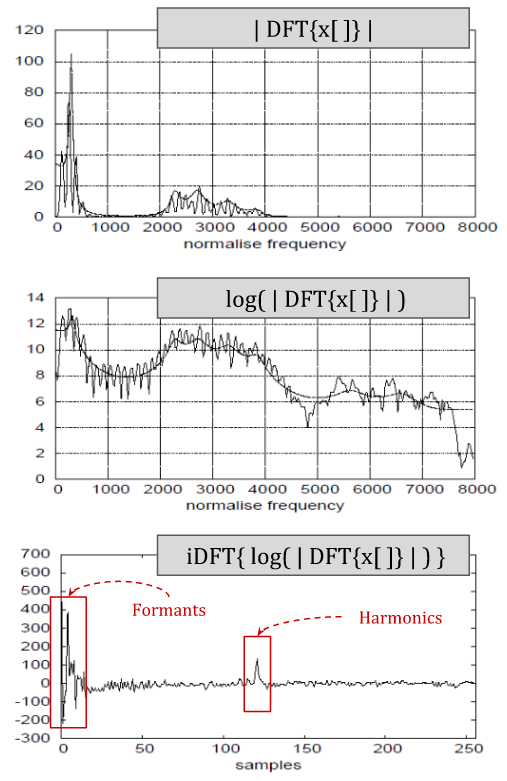
\includegraphics[width=0.6\textwidth]{bilder/cepstrum04.png}
	\caption{Berechnung des Cepstrums. (nach: \cite[Cepstral Analysis, S. 3]{ricardo_ceps})}
	\label{img:cepstrumOverview}
\end{figure}

Das Vorgehen wird mit Hilfe des Beispiels aus Abbildung \ref{img:cepstrumOverview} erläutert. $ |\ \text{DFT}\{x[\;]\} \big| $  zeigt das Spektrum eines \glqq typischen stimmhaften\grqq{} Signals $x[\;]$. Es sind die in Kapitel \ref{sec:theVoice} erläuterten für ein stimmhaftes Signal typischen harmonischen Obertöne zu sehen, welche mit steigender Frequenz an Amplitude verlieren. Durch das logarithmieren des Spektrums $\log \Big(\ \big|\ \text{DFT}\{x[\;]\} \big|\ \Big)$ wird die Dynamic des Frequenzbereiches verringert und somit der Amplitudenverlust der höheren Obertöne verringert. Nun stellt man sich vor, dieses Spektrum wäre ein Signal des Zeitbereiches. Dieses Signal würde man als ein annährend periodisches Signal mit einer Amplituden-Modulation interpretieren, das heißt ein Signal mit hoher Frequenz, addiert mit einem Signal mit nierdiger Frequenz. Um diese beiden Komponenten voneinander zu trennen, müsste man eine weitere DFT anwenden. Diese DFT kommt in dem Fall einer inversen DFT gleich, da das Phasen-Signal verworfen wurde. Man erwartet in diesem \glqq Spektrum vom Spektrum\grqq{} einen Peak im \glqq oberen Frequenzbereich\grqq , bedingt durch die harmonischen Oberwellen, sowie einen Peak im \glqq unteren Frequenzbereich\grqq, bedingt durch die Formanten.\cite[Cepstral analysis]{ricardo_ceps}

Der Bereich dieser \glqq Fouriertransformation der Fouriertransformation\grqq{} wird als \emph{Cepstrum} bezeichnet. Cepstrum ist ein ein Wortspiel, welches durch die Umkehrung der ersten vier Buchstaben des Wortes "Spectrum" entsteht. Die Unabhängige Variable des Cepstrum wird als \emph{Quefrency} bezeichnet. Damit wird verdeutlicht, dass die unabhängige Variable des Cepstrum zwar mathematisch betrachtet die Zeit darstellt, jedoch als Frequenz interpretiert wird.\cite[S. 7]{ricardo_ceps}

\begin{figure}[h]
	\centering
	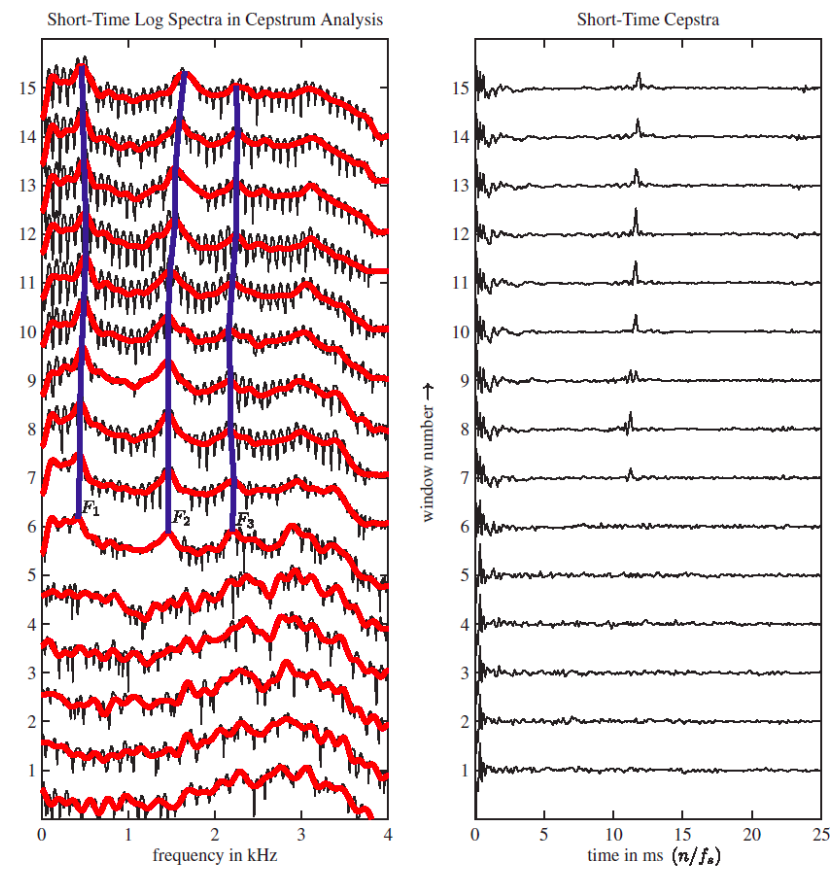
\includegraphics[width=0.6\textwidth]{bilder/cepstrum05.png}
	\caption{Aufkommen eines Peaks im oberen Quefrency-Bereich bei stimmhaften Signalfenstern. \cite[Cepstral Analysis, S. 17]{ricardo_ceps}}
	\label{img:cepstrumVoicedPeak}
\end{figure}	

Ein Auftauchen eines Peaks im oberen Quefrency-Bereich $> \SI{3}{\milli\second}$ spricht für das Vorhandensein von harmonischen Obertönen im Signal, wie sie durch Stimme erzeugt werden. Abbildung \ref{img:cepstrumVoicedPeak} verdeutlicht das Prinzip an einem Beispiel. Zu sehen ist die STFT eines Signals mit einer Fensterlänge von $\SI{50}{\milli\second}$ und einer Hopsize von $\SI{12.5}{\milli\second}$. Links wird das logarithmierte Spektrum abgebildet, rechts das Cepstrum. Die Frames 1 bis 5 sind stimmlos, die Frames 8 bis 15 sind stimmhaft, und die zwischen-Frames eine Mischung. Man sieht das Aufkommen eines Peaks bei einer Quefrency $q = \SI{12}{\milli\second}$.\cite[S. 16]{ricardo_ceps}

Abbildung \ref{img:cepstrumPitch} verdeutlicht, wie eine Grundfrequenz $f_0$ im Zeitbereich einen Peak im Cepstrum erzeugt. So weist ein Peak an bei der Quefrency $q$ auf eine Grundfrequenz von $f_0 = f_s/q$ hin.\cite{cepstrumPitchTranslation}

\begin{figure}[h]
	\centering
	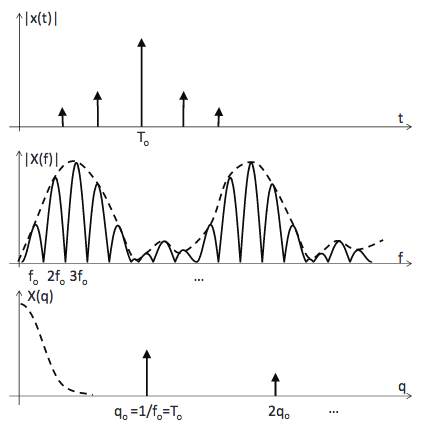
\includegraphics[width=0.6\textwidth]{bilder/cepstrumPitch.png}
	\caption{Feststellung der Grundfrequenz aus dem Cepstrum. \cite{cepstrumPitchTranslation}}
	\label{img:cepstrumPitch}
\end{figure}

In Bezug auf die Voice Activity Detection wurde das Cepstrum genutzt, um die beiden Features \emph{Obere Cepstrum-Spitze} [$Ceps_{mag}$] und \emph{Quefrency der oberen Cepstrum-Spitze} [$Ceps_{loc}$] zu berechnen.

Ahmadi et al. \cite{vad_ceps} sowie Kristjansson et al.\cite{vad_Lisboa} schlagen vor, die Höhe der Magnitude eines Peaks im oberen Bereich des Cepstrums als Maß für die Stimmhaftigkeit des Signals einzusetzen. Formel \ref{eq:ceps_maxpeak} definiert die Berechnung. $c_i[\;]$ ist das Cepstrum des $i$-ten Frequenzfensters $X_i[\;]$. Wie in Kapitel \ref{sec:acousticModel} erläutert, liegt die Grundfrequenz bei kindlichen Lautäußerungen zwischen 200 und \SI{2000}{\hertz}, was einem Quefrency-Bereich von 5 - \SI{40}{\milli\second} entspricht. Folglich werden bei der Berechnung nach Formel \ref{eq:ceps_maxpeak} nur Quefrency-Werte in diesem Bereich betrachtet. 

\begin{equation}
Ceps_{mag}(c_i[\;]) = \maxmagi_{q = q_{min} \ldots , q_{max}}\{ \; c[q] \; \}
\label{eq:ceps_maxpeak}
\end{equation}

Als zweites Attribut, welches auf dem Cesptrum basiert, wurde die Quefrency der höchsten Amplitude des oberen Cepstrum-Bereiches nach Formel \ref{eq:ceps_loc} berechnet. Bei Signalfenstern ohne Stimme ist es wahrscheinlicher, dass sich die höchste Amplitude am Mindest- oder Maximalwert des durchsuchten Quefrency-Bereiches befindet.

\begin{equation}
Ceps_{loc}(c_i[\;]) = \argmax \{ \; c[\;] \; \}
\label{eq:ceps_loc}
\end{equation}	

\subsubsection{Differenz-Feature}
\label{sec:vad_dif_feature}

Abbildung \ref{img:vadAllFeatures} visualisiert alle Attribute, die in den Kapiteln \ref{sec:vad_time_features} bis \ref{sec:vad_ceps_features} vorgestellt wurden. Der oberste Plot zeigt das Audiosignal aus Abbildung \ref{img:vad01} mit einem Signal/Rausch-Abstand von \SI{20}{\decibel}. Der rote Graph über dem Plot klassifiziert die Zeitbereiche in $1 \; \hat{=} $ \emph{stimmhaft} und $0 \; \hat{=}$ \emph{nicht stimmhaft}. Alle darunter liegenden Plots zeigen den zeitlichen Verlauf der entsprechenden Attribute.

\begin{figure}[h]
	\centering
	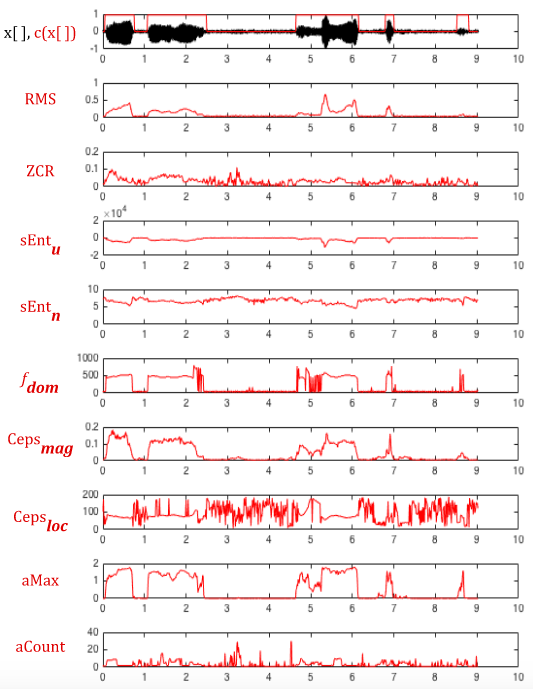
\includegraphics[width=0.85\textwidth]{bilder/allFeatures01.png}
	\caption{Übersicht über alle Features, die für die Voice Activity Detection erprobt wurden.}
	\label{img:vadAllFeatures}
\end{figure}

Abbildung \ref{img:min-signal} zeigt den zeitlichen Verlauf des RMS-Features im Detail. (A) zeigt das verhalten des \emph{RMS}-Attributes bei einem Signal/Rauschabstand von \SI{50}{\decibel}. Die stimmlosen Zeiträume haben einen weitaus niedrigeren RMS-Wert als die Zeiträume mit Stimme. In (B) ist das selbe Signal mit einem Signal/Rauschabstand von \SI{3}{\decibel} zu sehen. Nun liegen die RMS-Werte der stimmlosen Bereiche nur noch knapp unter denen des Sprachsignals. Zu sehen ist, dass starkes Hintergrundrauschen ähnlich hohe Feature-Werte erzeugen kann wie die Stimme.

\begin{figure}[h]
	\centering
	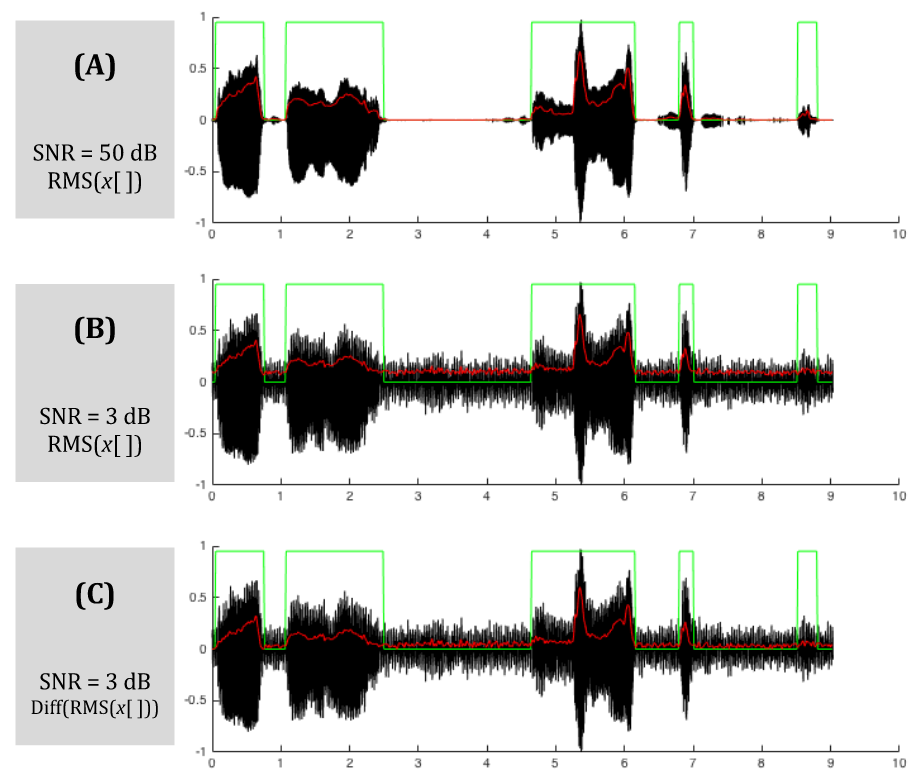
\includegraphics[width=0.7\textwidth]{bilder/rms_diff.png}
	\caption{Das RMS-Feature bei verschiedenen Signal/Rausch-Abständen. Schwarz: Eingangs-Signal $x[\;]$. Grün: Klassifizierung in Stimmhaft/Stille. Rot: Feature-Wert.}
	\label{img:min-signal}
\end{figure}

Moattar et al \cite{vad_Easy} und Waheed et al \cite{vad_entropy} präsentierten die Idee, den Wert des jeweiligen Attributes zu messen, der in den stimmlosen Bereichen durch das Hintergrundrauschen erzeugt wird. Es kann davon ausgegangen werden, dass die ersten Signalfenster eines Signals stimmlos sind, und der Feature-Wert des Rauschens somit anhand dieser Fenster bestimmt werden kann. Bei einer langanhaltenden und kontinuierlichen Analyse können sich sowohl der Signal/Rausch-Abstand als auch die Qualität des Rauschens ständig ändern, weshalb die von den stimmlosen Bereichen erzeugten Attributwerte regelmäßig aktualisiert werden müssen. Es kann weiterhin davon ausgegangen werden, dass die Länge einer Cry-Unit eine bestimmte Länge $t_{max}$ nicht überschreiten kann, bevor das Baby Luft holen muss und somit zumindest ein stimmloses Zeitfenster entsteht, welches das Hintergrundrauschen enthält. Zeskind et al. \cite[S. 325]{rythmic} haben $t_{max} = \SI{4.75}{\second}$ bestimmt. In einem Zeitbereich $ t > t_{max}$ muss somit zumindest ein Feature-Wert enthalten sein, der durch stimmlose Signalteile erzeugt wird. 

Auf Basis dieser Überlegung wurde das \emph{Differenz-Feature} Diff\textsubscript{t}(\text{Feat}$(x_i[\;])$) nach Formel \ref{eq:difFeature} definiert als die Differenz zwischen einem aktuell gemessenen Attributwerte und dem geringsten Attributwerte, welcher im vergangenen Zeitbereich $t$ gemessen wurde. Feat$(x_i[\;])$ bezeichnet dabei einen beliebigen Feature-Wert des Signalfensters $x_i[\;]$, $t_{xi}$ die Länge eines Signalfensters in Sekunden (in diesem Fall \SI{25}{\milli\second}), und $t$ der in der Vergangenheit zu durchsuchende Zeitbereich in Sekunden $> t_{max}$. In Abbildung \ref{img:min-signal} wird in (C) das Differenz-Feature für den RMS-Wertes gezeigt.

\begin{equation}
\text{Diff}_t(\text{Feat}(x_i[\;])) = \text{Feat}(x_i[\;])\ - \mini_{k=i-z...i}\{\text{Feat}(x_k[\;])\}, \qquad z = \frac{2 \cdot t}{t_{xi}}
\label{eq:difFeature}
\end{equation}

In dieser Arbeit wurde $t = \SI{5}{\second}$ festgelegt. Es ist zu beachten, dass die Attribute \emph{ZCR, SEnt\textsubscript{u}} und \emph{aCount} zur Berechnung des Differenz-Features bezüglich ihres Vorzeichens invertiert werden müssen, da bei Ihnen ein niedriger an Stelle eines hohen Wertes stimmhafte Signale anzeigen. Das einzige Attribut, für dass die Berechnung des Differenz-Features keinen Sinn macht, ist das \emph{Ceps\textsubscript{loc}}-Attribut, da es bei stimmlosen Signalabschnitten sowohl einen höheren als auch einen niedrigeren Wert annehmen kann.

\subsubsection{Entscheidung}

Die einfachste Variante zur Entscheidung, ob ein Signalfenster $x_i[\;]$ stimmhaft ist, ist, eines der vorgestellten Features als Entscheidungsgrundlage zu wählen und einen festen Grenzwert $\theta$ festzulegen, bei dessen Über- oder Unterschreitung das Fenster als Stimmhaft klassifiziert wird. Die Entscheidung lässt sich als Klassifizierungsfunktion $C$, welche ein Signalfenster abbildet auf $Y = \{ 1 \; \hat{=} \; \text{stimmhaft}, 0 \; \hat{=} \; \text{nicht stimmhaft}\}$, das heißt $C(x[\;]) \mapsto \{1,0\}$. Die Klassifzierungsfunktion nimmt dann die folgende Form an:

\begin{equation}
	C(x_i[\;]) = 
\begin{cases}
1 \quad , \text{wenn Feat}(x_i[\;]) > \theta \\
0 \quad , \text{sonst}
 \end{cases}
\end{equation}

 Abbildung \ref{img:thresholded} verdeutlicht das Prinzip an einem Beispiel. Das Feature, dass als Entscheidungsgrundlage genutzt wird, ist der \emph{RMS}-Wert. Ein Grenzwert von $\theta = 0.18$ würde in diesem Fall eine weitestgehend richtige Klassifizierung gewährleisten.

\begin{figure}[h]
	\centering
	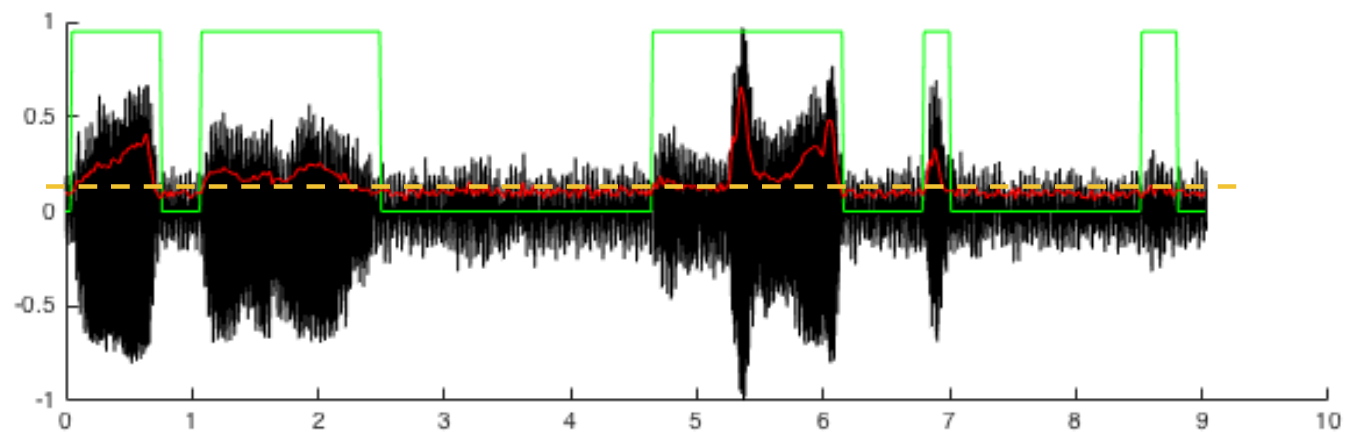
\includegraphics[width=0.6\textwidth]{bilder/thresholded02.png}
	\caption{Thresholding eines Features. Schwarz: Das Eingangssignal $x[\;]$. Grün: Klassifizierung in Stimmhaft/Stille. Rot: RMS-Feature. Orange: Grenzwert}
	\label{img:thresholded}
\end{figure}

Die Frage ist, wie man diesen Grenzwert findet. Einige Veröffentlichungen, so wie die von Moattar et al. \cite{vad_Easy} empfehlen, den Grenzwert experimentell festzustellen. In dieser Arbeit wurde sich für den Ansatz einer automatisierten, datengetriebenen Suche der Grenzwerte mit Hilfe des in Kapitel \ref{sec:id3} vorgestellten \emph{C4.5}-Algorithmus entschieden. Der Grundgedanke ist wie folgt: Angenommen, man hat einen Trainingsdatensatz zur Verfügung, bestehend aus einer Menge an Signalen mit Aufnahmen von kindlichen Lautäußerungen, in denen manuell die stimmhaften Signalabschnitte markiert wurden. Diese Signale zerlegt man nach den besprochenen Methoden in kürzere Signalfenster und berechnet für jedes Signalfenster das Feature, dessen Grenzwert man sucht. Jedem Signalfenster versieht man außerdem mit dem Klassenlabel $y \in Y$ auf Basis der manuellen Markierungen. Ein \emph{Signalfenster} $x_i[\;]$ wird so zu einer \emph{Instanz} $(\text{Feat}(x_i[\;]), y_i)$. Nun kann der \emph{C4.5}-Algorithmus verwendet werden, um für ein Feature den Grenzwert zu finden, der für diese Datenbasis die Klassifizierung mit der höchsten Genauigkeit vornimmt. Voraussetzung dafür ist, dass der \emph{C4.5}-Algorithmus gezwungen wird, einen Entscheidungsbaum mit einer maximalen Tiefe von $1$ zu erzeugen, damit auch nur ein Grenzwert gesucht wird. Ist das Feature, für das der Grenzwert gesucht wird, ein Differenz-Feauture (siehe Kapitel \ref{sec:vad_dif_feature}), so lässt sich dieser Grenzwert als ein adaptiver Grenzwert interpretieren, der sich an den aktuellen SNR anpasst.

Die Verwendung des \emph{C4.5}-Algorithmus bringt die Möglichkeit mit sich, eine beliebige Menge an Features in die Klassifizierung mit einzubeziehen. Die Klassifizierung muss also nicht zwingend auf Grundlage nur eines Attributes geschehen. Angenommen, es werden die Features Ceps$_{mag}$ und der RMS-Wert für jedes Signalfenster berechnet. Der \emph{C4.5}-Algorithmus würde nun für einen Trainingsdatensatz einen Entscheidungsbaum konstruieren, bei dem durch das hierarchische Setzen von Grenzwerten die Klassifikation vorgenommen wird. Listing \ref{lst:tree01} zeigt ein Beispiel für eine so möglicherweise resultierende Klassifzierungsfunktion.

\begin{lstlisting}[frame=single,mathescape=true,basicstyle=\footnotesize,language=Java,label=lst:tree01,caption=Beispiel eines CART-Entscheidungsbaums,linewidth=1\textwidth]
if Ceps$_{mag}$($x_i[\;]$) > 0.2
|   if RMS($x_i[\;]$) < 0.13
|   |   C($x_i[\;]$) = 0
|   |else
|   |   C($x_i[\;]$) = 1
|else
|    C($x_i[\;]$) = 1
\end{lstlisting}

Wird dem \emph{C4.5}-Algorithmus eine größere Menge an Attributen zur Verfügung gestellt, auf deren Basis der Klassifikator entworfen wird, wird der Entscheidungsbaum implizit zeigen, welche Features für die VAD besser geeignet sind, da sie höher im Entscheidungsbaum stehen werden. Es besteht jedoch immernoch die Gefahr, dass der Klassifikator in ein lokales Maximum gelaufen ist und eine suboptimale Auswahl an Features durch den Algorithmus getroffen wurde. Außerdem besteht die Gefahr von Overfitting, insofern Entscheidungsbäume mit beliebiger Tiefe zugelassen werden.

\subsection{Simulations-Studie}
\label{sec:vad_study}

\subsubsection{Datenbank}

\subsection{Konstruktion des Featureraumes}

\subsubsection{Grenzwertfindung durch den C4.5}

\subsection{Ergebnisse}
\label{sec:vad_results}

\section{Markierung der Cry-Units}
\label{sec:marking_cry-units_new}

\section{Decision Smoothing}
\label{sec:decision_smoothing_new}





